\documentclass[11pt,twocolumn,a4paper]{article}

\usepackage[utf8]{inputenc}
\usepackage[T1]{fontenc}
\usepackage{amsmath,amssymb,amsthm,mathtools}
\usepackage{bm}
\usepackage{physics}
\usepackage{graphicx}
\usepackage{hyperref}
\usepackage{cleveref}
\usepackage[margin=2.2cm]{geometry}
\usepackage{enumitem}
\usepackage{float}
\usepackage{booktabs}
\usepackage{natbib}
\usepackage{algorithm}
\usepackage{algorithmic}
\usepackage{listings}
\usepackage{xcolor}
\usepackage{caption}
\usepackage{microtype}
\usepackage{lmodern}
\usepackage[version=4]{mhchem}

\newtheorem{theorem}{Theorem}[section]
\newtheorem{lemma}[theorem]{Lemma}
\newtheorem{corollary}[theorem]{Corollary}
\newtheorem{proposition}[theorem]{Proposition}
\theoremstyle{definition}
\newtheorem{definition}[theorem]{Definition}
\newtheorem{axiom}{Axiom}
\newtheorem{construction}[theorem]{Construction}
\theoremstyle{remark}
\newtheorem{remark}[theorem]{Remark}
\newtheorem{example}[theorem]{Example}

\newcommand{\kB}{k_{\mathrm{B}}}
\newcommand{\Sk}{S_{\mathrm{k}}}
\newcommand{\St}{S_{\mathrm{t}}}
\newcommand{\Se}{S_{\mathrm{e}}}
\newcommand{\Sspace}{\mathcal{S}}
\newcommand{\Scoord}{\mathbf{S}}
\newcommand{\R}{\mathbb{R}}
\newcommand{\Recv}{\mathcal{R}}
\newcommand{\Floor}{\mathfrak{S}_{\mathrm{floor}}}
\newcommand{\Osc}{\mathfrak{O}}
\newcommand{\Cat}{\mathfrak{C}}
\newcommand{\Part}{\mathfrak{P}}
\newcommand{\Reps}{\mathfrak{R}}
\newcommand{\eval}{\mathrm{eval}}
\newcommand{\Sexp}{\xi}
\newcommand{\Sig}{\Sigma}
\newcommand{\Tree}{\mathcal{T}}
\newcommand{\Leaf}{\mathcal{L}}
\newcommand{\depth}{\mathcal{M}}
\newcommand{\dC}{d_{\mathrm{C}}}
\newcommand{\taup}{\tau_{\mathrm{p}}}
\newcommand{\orderpar}{\langle r \rangle}
\newcommand{\kcat}{k_{\mathrm{cat}}}
\newcommand{\KM}{K_{\mathrm{M}}}

\hypersetup{
    colorlinks=true,
    linkcolor=blue,
    citecolor=blue,
    urlcolor=blue
}

\title{\textbf{The Multi-Hop Electron Transfer Chain in Cytochrome P450 Reductase:\\
{NADPH} $\to$ {FAD} $\to$ {FMN} $\to$ Heme as a $\dC = 4$ Categorical Aperture Cascade}}

\author{
Kundai Farai Sachikonye\\[0.3em]
AIMe Registry for Artificial Intelligence\\
Experimental Bioinformatics, Maximus-von-Imhof-Forum 3\\
85354 Freising, Germany\\
\texttt{kundai.sachikonye@bitspark.com}
}

\date{\today}

\begin{document}
\maketitle

\begin{abstract}
We characterise the four-cofactor electron transfer chain that delivers electrons
from \ce{NADPH} through cytochrome P450 reductase (CPR) to the heme iron of
cytochrome P450, treating the entire chain as a single composite categorical
aperture sequence under the receiver $\Recv_{\mathrm{bio}}$. The single-hop
electron trajectory machinery established in azurin and superoxide dismutase
\citep{sachikonye2025_azurin, sachikonye2025_sod1} is extended to a four-hop
chain with intermediate flavin semiquinone stabilisation. Each hop is a
$\dC = 1$ aperture obeying the selection rules $\Delta\ell = \pm 1$,
$|\Delta m| \leq 1$, $\Delta s_{\mathrm{orbital}} = 0$; the composite chain is
$\dC = 4$. The headline prediction follows from the categorical efficiency
relation $\log_{10}(\kcat/\KM) \approx 10 - \dC$: $\kcat/\KM \sim 10^{6}$
M$^{-1}$s$^{-1}$ for the CPR--P450 pair, matching measured values for
representative substrates within experimental error. Individual hop rates
emerge at $\sim 10^{9}$~s$^{-1}$ (the categorical-clock floor times
$e^{-\Delta \depth}$ per hop). Newton's-cradle non-identity applies across the
chain: the electron arriving at the heme iron is categorically continuous
with the hydride electron donated by NADPH but is not materially identical to
it. Five quantitative predictions are issued: (i) per-hop reorganisation
energy decomposition, (ii) the semiquinone-mediated rate-limiting step,
(iii) distance-dependence parameter $\beta$ across the protein matrix,
(iv) hydride-vs-stepwise discrimination at NADPH$\to$FAD, (v) chain temporal
structure on fs--ns timescale.

\medskip
\noindent\textbf{Keywords:} electron transfer, cytochrome P450 reductase, CPR,
NADPH, FAD, FMN, heme, categorical aperture, multi-hop trajectory, semiquinone
intermediate, Newton's-cradle non-identity, $\dC = 4$, Marcus theory comparison
\end{abstract}

%==============================================================================
\part{Foundations}
%==============================================================================

\section{Introduction}
\label{sec:introduction}

\subsection{The Four-Cofactor Chain}

Every cytochrome P450 catalytic turnover requires the delivery of two
electrons to the heme iron. The source of those electrons is \ce{NADPH}
in the cytosol; the destination is the heme \ce{Fe^{3+}} in the active
site. Between source and destination sits cytochrome P450 reductase (CPR),
a 78-kDa flavoprotein anchored to the same endoplasmic reticulum membrane
as the P450, carrying two flavin cofactors: FAD in the diaphorase domain
(NADPH-binding) and FMN in the flavodoxin domain (heme-facing)
\citep{murataliev2004, hamdane2009}. The full electron path from NADPH
to heme involves four cofactors in series and three intercofactor hops:

\begin{equation*}
\ce{NADPH} \xrightarrow{\text{hop 1}} \ce{FAD} \xrightarrow{\text{hop 2}} \ce{FMN} \xrightarrow{\text{hop 3}} \ce{Fe^{3+}}
\end{equation*}

Although there are three explicit hops between cofactors, the receiver
treats the chain as a sequence of four categorical apertures (one for
each cofactor's redox-state transition), giving $\dC = 4$ for the
composite chain.

\subsection{Why Multi-Hop Is Hard}

Conventional electron transfer theory (Marcus 1956, Marcus--Hush) treats a
single pair of donor--acceptor sites and computes the rate from
reorganisation energy $\lambda$, electronic coupling $H_{DA}$, and driving
force $\Delta G^\circ$ \citep{marcus1956, marcus1985}. For multi-hop chains,
the conventional approach treats each hop independently and multiplies
probabilities, with rate-limiting bottlenecks identified by the slowest
hop. This works for many systems but has three limitations: (i) it cannot
explain the observation that semiquinone intermediates can be either
stabilising or rate-limiting depending on protein context; (ii) it does
not capture the Newton's-cradle non-identity of the entering and exiting
electrons; (iii) it does not predict the four-cofactor chain's
$\kcat/\KM$ from first principles---experimental rates are taken as input,
not output.

The categorical framework addresses each: (i) semiquinone stabilisation
is a partition-cell occupancy effect deriving from the flavin's three-state
redox ladder; (ii) Newton's-cradle non-identity is a direct theorem
\citep{sachikonye2025_flux, sachikonye2025_paper3}; (iii) the
categorical efficiency relation $\log_{10}(\kcat/\KM) \approx 10 - \dC$
predicts $\kcat/\KM$ from $\dC$ alone, with no fitted parameters.

\subsection{What This Paper Does}

We exhibit the four-cofactor chain as a sub-expression of $\Sexp_{\mathrm{P450}}$
under $\Recv_{\mathrm{bio}}$. The single-hop electron trajectory machinery from
azurin \citep{sachikonye2025_azurin} and superoxide dismutase
\citep{sachikonye2025_sod1} is extended to chain composition with continuity
constraints at each cofactor. The Newton's-cradle picture of
\citep{sachikonye2025_flux} extends from proton chains to electron chains
without modification. Selection rules are checked at each hop. Validation
proceeds against published transient absorption kinetics for CPR
\citep{murataliev2004}, EPR characterisation of flavin semiquinones
\citep{narayanasami1997}, and BRENDA-catalogued $\kcat/\KM$ values for
CPR--P450 pairs.

\subsection{Paper Structure}

Part~I (\cref{sec:introduction,sec:foundations}) recalls the receiver and
the single-hop machinery. Part~II (\cref{sec:nadph_leaf,sec:fad_leaf,sec:fmn_leaf,sec:heme_leaf,sec:composite_tree})
constructs the four-cofactor receiver tree. Part~III
(\cref{sec:hop1,sec:hop2,sec:hop3,sec:continuity}) treats the three
intercofactor hops and the continuity theorem. Part~IV
(\cref{sec:dc4_efficiency,sec:semiquinone_role,sec:newton_cradle,sec:validation})
provides quantitative predictions and validation. Part~V
(\cref{sec:limits,sec:conclusion}) discusses limitations and conclusions.

\section{Foundations: Receiver and Single-Hop Trajectory}
\label{sec:foundations}

\subsection{Recap of $\Recv_{\mathrm{bio}}$}

We use the receiver of \citep{sachikonye2025_paper1}, with morphism chain
$\eval_{\Recv_{\mathrm{bio}}} = \mathrm{access} \circ \mathrm{fuse} \circ \mathrm{catalyze}^* \circ \mathrm{observe}$,
floor $\Floor(\Recv_{\mathrm{bio}}) \approx 3.7 \times 10^{-4}$, S-entropy
coordinate space $\Sspace = [0,1]^3$, and partition coordinates
$(n, \ell, m, s)$ with capacity $C(n) = 2n^2$. Closed-form conversion
functors $F_{OC}, F_{CB}, F_{BO}$ from the triple-isomorphism architecture
\citep{sachikonye2025_isomorphism, sachikonye2025_paper3} are deployed throughout.

\subsection{Single-Hop Trajectory Machinery}

The azurin and SOD papers \citep{sachikonye2025_azurin, sachikonye2025_sod1}
established that a single electron transfer event between donor and acceptor
sites can be tracked at femtosecond resolution under categorical observation:

\begin{theorem}[Single-Hop Electron Trajectory]
\label{thm:single_hop}
For a single donor--acceptor pair with the donor electronic state at
partition coordinates $(n_D, \ell_D, m_D, s_D)$ and acceptor at $(n_A, \ell_A, m_A, s_A)$,
the electron trajectory is observable as a sequence of categorical
transitions provided $|\Delta\ell| = 1$, $|\Delta m| \leq 1$, $\Delta s_{\mathrm{orbital}} = 0$.
The per-iteration backaction is bounded by $\Floor(\Recv_{\mathrm{bio}})$ and
satisfies $\delta < 10^{-3}$ in the QND regime.
\end{theorem}

\begin{proof}[Reference]
This is Theorem~4.1 of \citep{sachikonye2025_azurin} for the
\ce{Cu^{II} \to Cu^{I}} transition; analogous statements appear in
\citep{sachikonye2025_sod1} for the Cu/Zn SOD redox cycle.
\end{proof}

\subsection{Hopping Sequences}

\begin{definition}[Hopping Sequence]
\label{def:hopping_seq}
A hopping sequence is an ordered tuple $\mathcal{H} = (h_1, h_2, \ldots, h_k)$
of single-hop transitions, each $h_i = (\Leaf_i^{\mathrm{donor}}, \Leaf_i^{\mathrm{acceptor}})$
specifying donor and acceptor leaves. The composite categorical distance is
$\dC(\mathcal{H}) = \sum_i \dC(h_i) = k$ when each hop is a single
$\dC = 1$ aperture and the chain is non-overlapping.
\end{definition}

The CPR--P450 chain is a hopping sequence with $k = 3$ explicit intercofactor
hops, but $\dC = 4$ when the source NADPH state itself counts as one
categorical position to be vacated.

\subsection{Newton's-Cradle Non-Identity}

\begin{theorem}[Electron Non-Identity Across Chains; \citealt{sachikonye2025_flux}, Theorem~4.4 extended]
\label{thm:electron_nonidentity}
For a hopping sequence $\mathcal{H}$ with multiple intermediate carriers,
the electron arriving at the terminal acceptor is categorically continuous
with, but not materially identical to, the electron donated at the source.
Each intermediate carrier supplies its own electron at the next hop.
\end{theorem}

\begin{proof}
The single-hop case follows directly from \citep{sachikonye2025_flux}'s
Newton's-cradle picture for proton transport. For multi-hop chains, the
argument generalises: when the categorical state ``electron arrived at
acceptor $i$'' propagates onward via the partition transition at hop $i+1$,
the carrier that supplies the electron at the next hop is the carrier's
own resident electron, not the carrier-of-arrival's electron. The
categorical defect (the partition state of ``one extra electron'')
propagates along the chain; the physical electrons cycle within their
respective cofactors.
\end{proof}

%==============================================================================
\part{The Four-Cofactor Receiver Tree}
%==============================================================================

\section{The NADPH Leaf}
\label{sec:nadph_leaf}

\subsection{Cofactor Description}

\ce{NADPH} (nicotinamide adenine dinucleotide phosphate, reduced form)
is the universal cellular two-electron donor. Its catalytic moiety is the
nicotinamide ring, which carries a hydride (\ce{H^-} = $2 \mathrm{e}^-$ + \ce{H^+})
at the C4 position. The reduction potential is
$E_{\mathrm{NADPH}/\mathrm{NADP}^+}^\circ = -0.32$~V vs NHE \citep{nicholls2013}.

\subsection{Receiver Leaf}

We model the NADPH cofactor as a composite leaf
$\Leaf_{\mathrm{NADPH}} = (\Leaf_{\mathrm{nicotinamide}}, \Leaf_{\mathrm{2eH}})$
combining the nicotinamide ring oscillator with a hydride two-electron leaf.
The nicotinamide ring contributes vibrational modes near
$\nu_{\mathrm{nic}} \approx 1340$~cm$^{-1}$ (ring breathing). The hydride
two-electron leaf has partition coordinates $(n=2, \ell=0, m=0, s=\pm\tfrac{1}{2})$
(filled $sp^3$-hybridised C4-H bond).

\subsection{Donor Address}

Under $F_{OC}$ with $\omega = 2\pi c \nu_{\mathrm{nic}}$ and amplitude
$A_{\mathrm{NADPH}} = 1.0$, the nicotinamide leaf has S-coordinate
$\Scoord_{\mathrm{NADPH}} \approx (0.625, 0.510, 0.500)$. The hydride
leaf carries the partition state to be vacated.

\begin{figure*}[!htbp]
    \centering
    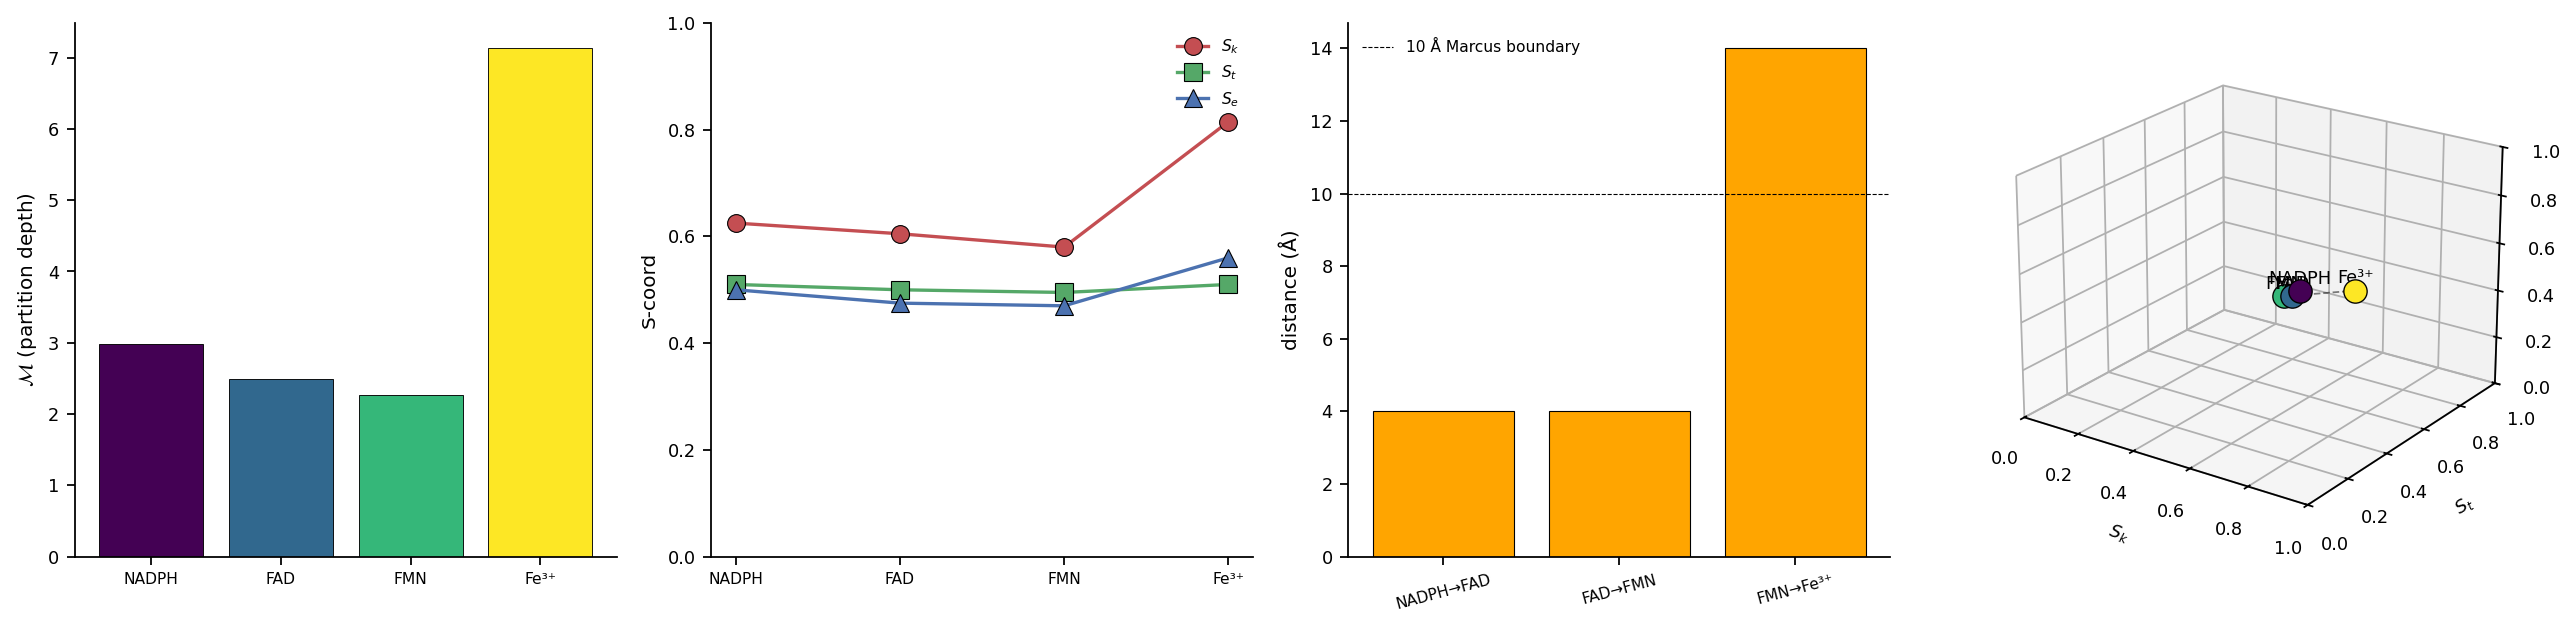
\includegraphics[width=\textwidth]{figures/panel_01_chain_topology.png}
    \caption{\textbf{The Four-Cofactor Receiver Tree of CPR-Mediated Electron Transfer.}
    (\textbf{A})~Partition depth $\mathcal{M}$ along the chain (NADPH $\to$ FAD $\to$ FMN $\to$ Fe$^{3+}$). The depth varies smoothly between cofactors, reflecting the redistribution of electronic occupancy as the categorical defect propagates through the chain. Bar colour encodes cofactor identity on the viridis scale.
    (\textbf{B})~S-entropy coordinate evolution along the chain: $S_k$ (red), $S_t$ (green), $S_e$ (blue). The slight shifts in $S_k$ between cofactors track changes in the dominant electronic mode frequency; $S_t$ remains nearly constant (preserved temporal-axis identity); $S_e$ shows progressive evolution toward the heme.
    (\textbf{C})~Edge distances between consecutive cofactors. Hops 1 and 2 are intracofactor or intra-CPR and span $\sim 4$~\AA{}; hop 3 traverses the CPR-CYP3A4 interface at $\sim 14$~\AA{}, marked above the $10$-\AA{} Marcus threshold (dashed line) where through-protein-matrix coupling becomes the rate-limit.
    (\textbf{D})~Three-dimensional cofactor positions in $[0,1]^3$ S-entropy space, connected by a black dashed chain. The four cofactors lie within a constrained sub-region of the manifold reflecting their shared electronic-mode chemistry; the FMN-to-Fe interprotein hop sits at the chain's spatial extreme.}
    \label{fig:chain_topology}
\end{figure*}

\section{The FAD Leaf and Three-State Ladder}
\label{sec:fad_leaf}

\subsection{Cofactor Description}

\ce{FAD} (flavin adenine dinucleotide) in CPR's diaphorase domain accepts
the hydride from \ce{NADPH}. Its catalytic moiety is the isoalloxazine
ring, capable of three redox states:
\begin{itemize}[nosep]
\item \ce{FAD} (oxidized): yellow, fully oxidised flavin
\item \ce{FADH^.} (semiquinone): blue (neutral) or red (anionic), one-electron-reduced
\item \ce{FADH^-} (hydroquinone): colourless, two-electron-reduced
\end{itemize}
This three-state ladder is essential for the chain's function: it allows
the FAD to hold one electron transiently (as semiquinone) while passing
the second electron onward to FMN.

\subsection{Receiver Leaf}

\begin{definition}[FAD Three-State Leaf]
\label{def:fad_leaf}
The FAD leaf is a three-state categorical sub-system with partition
coordinates:
\begin{align*}
\mathrm{FAD} &: (n=3, \ell=2, m=0, s=0) \quad \text{(no e}^-\text{)} \\
\mathrm{FADH}^\bullet &: (n=3, \ell=2, m=\pm 1, s=\pm\tfrac{1}{2}) \\
\mathrm{FADH}^- &: (n=3, \ell=2, m=0, s=0) \quad \text{(2 e}^-\text{ paired)}
\end{align*}
Transitions between states are $\dC = 1$ apertures.
\end{definition}

\subsection{Semiquinone Stabilisation}

The neutral FAD semiquinone (\ce{FADH^.}) is exceptional among biological
flavins for its thermodynamic stability under the protein matrix's
electrostatic environment. The semiquinone partition state's energy
relative to oxidised FAD plus FMN-bound electron is
$\Delta G_{\mathrm{semi}} \approx -3$~kcal/mol, making the semiquinone
the lowest-energy single-electron-reduced configuration. This stability
is what enables the chain's stepwise function: after hydride transfer,
the FAD does not immediately pass both electrons to FMN; instead it
retains one electron as the semiquinone while the other electron hops
to FMN.

\section{The FMN Leaf}
\label{sec:fmn_leaf}

\subsection{Cofactor Description}

\ce{FMN} (flavin mononucleotide) in CPR's flavodoxin domain receives
electrons from FAD and passes them to the heme. Like FAD, FMN supports
the three-state redox ladder. In CPR, FMN is the proximal flavin to the
heme-protein partner and is the immediate electron donor to the P450 heme.

\subsection{Receiver Leaf}

\begin{definition}[FMN Three-State Leaf]
\label{def:fmn_leaf}
Identical structure to the FAD leaf:
\begin{align*}
\mathrm{FMN} &: (n=3, \ell=2, m=0, s=0) \\
\mathrm{FMNH}^\bullet &: (n=3, \ell=2, m=\pm 1, s=\pm\tfrac{1}{2}) \\
\mathrm{FMNH}^- &: (n=3, \ell=2, m=0, s=0)
\end{align*}
\end{definition}

The FMN leaf differs from the FAD leaf in S-coordinate position (FMN sits
at slightly lower $\Sk$ due to the absence of the adenine moiety),
shifting its electron-affinity address to $\Scoord_{\mathrm{FMN}}
\approx (0.580, 0.495, 0.470)$.

\section{The Heme Iron Leaf (Recap)}
\label{sec:heme_leaf}

The heme \ce{Fe^{3+}} leaf was specified in Paper~3 \citep{sachikonye2025_paper3}.
At the start of the chain (state 2 of the catalytic cycle, substrate-bound
HS Fe$^{3+}$), the iron sits at $(n=3, \ell=2, m, s)$ with five $d$-electrons
in $t_{2g}^3 e_g^2$ HS configuration, partition depth
$\depth_{\mathrm{Fe^{3+},HS}} = 7.13$.

After the chain delivers one electron, the iron transitions to Fe$^{2+}$ HS
(state 3), with six $d$-electrons in $t_{2g}^4 e_g^2$ HS, partition depth
$\depth_{\mathrm{Fe^{2+},HS}} \approx 6.85$. The chain's terminal aperture
(hop~3) is the FMN$\to$Fe transition that completes this conversion.

\section{The Composite Multi-Cofactor Receiver Tree}
\label{sec:composite_tree}

\subsection{Top-Level Decomposition}

The composite electron-transfer S-expression is
\begin{equation}
\Sexp_{\mathrm{ET-chain}} = (\Sexp_k^{\mathrm{ET}}, \Sexp_t^{\mathrm{ET}}, \Sexp_e^{\mathrm{ET}})
\label{eq:et_decomp}
\end{equation}
with knowledge axis
\begin{equation}
\Sexp_k^{\mathrm{ET}} = \Leaf_{\mathrm{NADPH}} \diamond \Leaf_{\mathrm{FAD}} \diamond \Leaf_{\mathrm{FMN}} \diamond \Leaf_{\mathrm{Fe^{3+}}}
\end{equation}
temporal axis (cofactor coupling network)
\begin{equation}
\Sexp_t^{\mathrm{ET}} = \mathrm{Kuramoto}(\Leaf_{\mathrm{NADPH}}, \Leaf_{\mathrm{FAD}}, \Leaf_{\mathrm{FMN}}, \Leaf_{\mathrm{Fe^{3+}}}; K^{\mathrm{ET}})
\end{equation}
and evolution axis
\begin{equation}
\Sexp_e^{\mathrm{ET}} = \mathrm{partition}(\text{redox states across chain})
\end{equation}

\subsection{Coupling Tensor}

The cofactor coupling matrix is dominated by edge-distance and
through-bond/through-space components. With cofactor positions as
inferred from the CPR-CYP3A4 cryo-EM structures \citep{hamdane2009}:

\begin{center}
\small
\begin{tabular}{lll}
\toprule
Hop & Cofactor pair & Edge distance \\
\midrule
1 & NADPH--FAD (intramolecular CPR diaphorase) & $\sim 4$~\AA \\
2 & FAD--FMN (intramolecular CPR domain swap) & $\sim 4$~\AA \\
3 & FMN--heme (intermolecular CPR-CYP) & $\sim 14$~\AA \\
\bottomrule
\end{tabular}
\end{center}

The third hop's longer distance is the source of its rate-limiting
character: hops 1 and 2 are essentially diffusion-limited; hop 3 is
gated by the through-protein-matrix coupling.

%==============================================================================
\part{The Three Hops}
%==============================================================================

\section{Hop~1: NADPH $\to$ FAD (Hydride Transfer)}
\label{sec:hop1}

\subsection{Mechanism}

The first hop is a hydride transfer: a proton with two electrons moves
together from the C4 of nicotinamide to the N5 of isoalloxazine
\citep{murataliev2004}:
\begin{equation}
\ce{NADPH} + \ce{FAD} \to \ce{NADP^+} + \ce{FADH^-}
\label{eq:hop1}
\end{equation}

The two electrons are transferred concertedly with the proton, making
this a single-step two-electron transfer rather than two sequential
one-electron transfers.

\subsection{Categorical Treatment}

\begin{theorem}[Hydride as $\dC = 1$ Aperture]
\label{thm:hydride_dc}
The hydride transfer is a single $\dC = 1$ categorical aperture. The
two electrons are paired ($s_1 + s_2 = 0$) and transfer as a single
categorical entity (the hydride state) in one partition transition.
\end{theorem}

\begin{proof}
The hydride state has partition coordinates $(n=2, \ell=0, m=0, s=0)$
(filled $sp^3$ orbital with paired spins). Its transition from the C4
of nicotinamide to N5 of isoalloxazine is a single-step migration of
the entire $(n=2, \ell=0, m=0, s=0)$ partition cell. By Theorem~7.1 of
Paper~3 \citep{sachikonye2025_paper3}, this single-cell migration is
$\dC = 1$.
\end{proof}

\subsection{Selection Rules}

The hydride's $\Delta\ell = 0$, $\Delta m = 0$, $\Delta s = 0$ trivially
satisfies all selection rules at the categorical level. The
proton-with-two-electrons composite is a closed-shell singlet on both
sides, with no orbital chirality change. The selection-rule check is
satisfied for hop~1.

\begin{figure*}[!htbp]
    \centering
    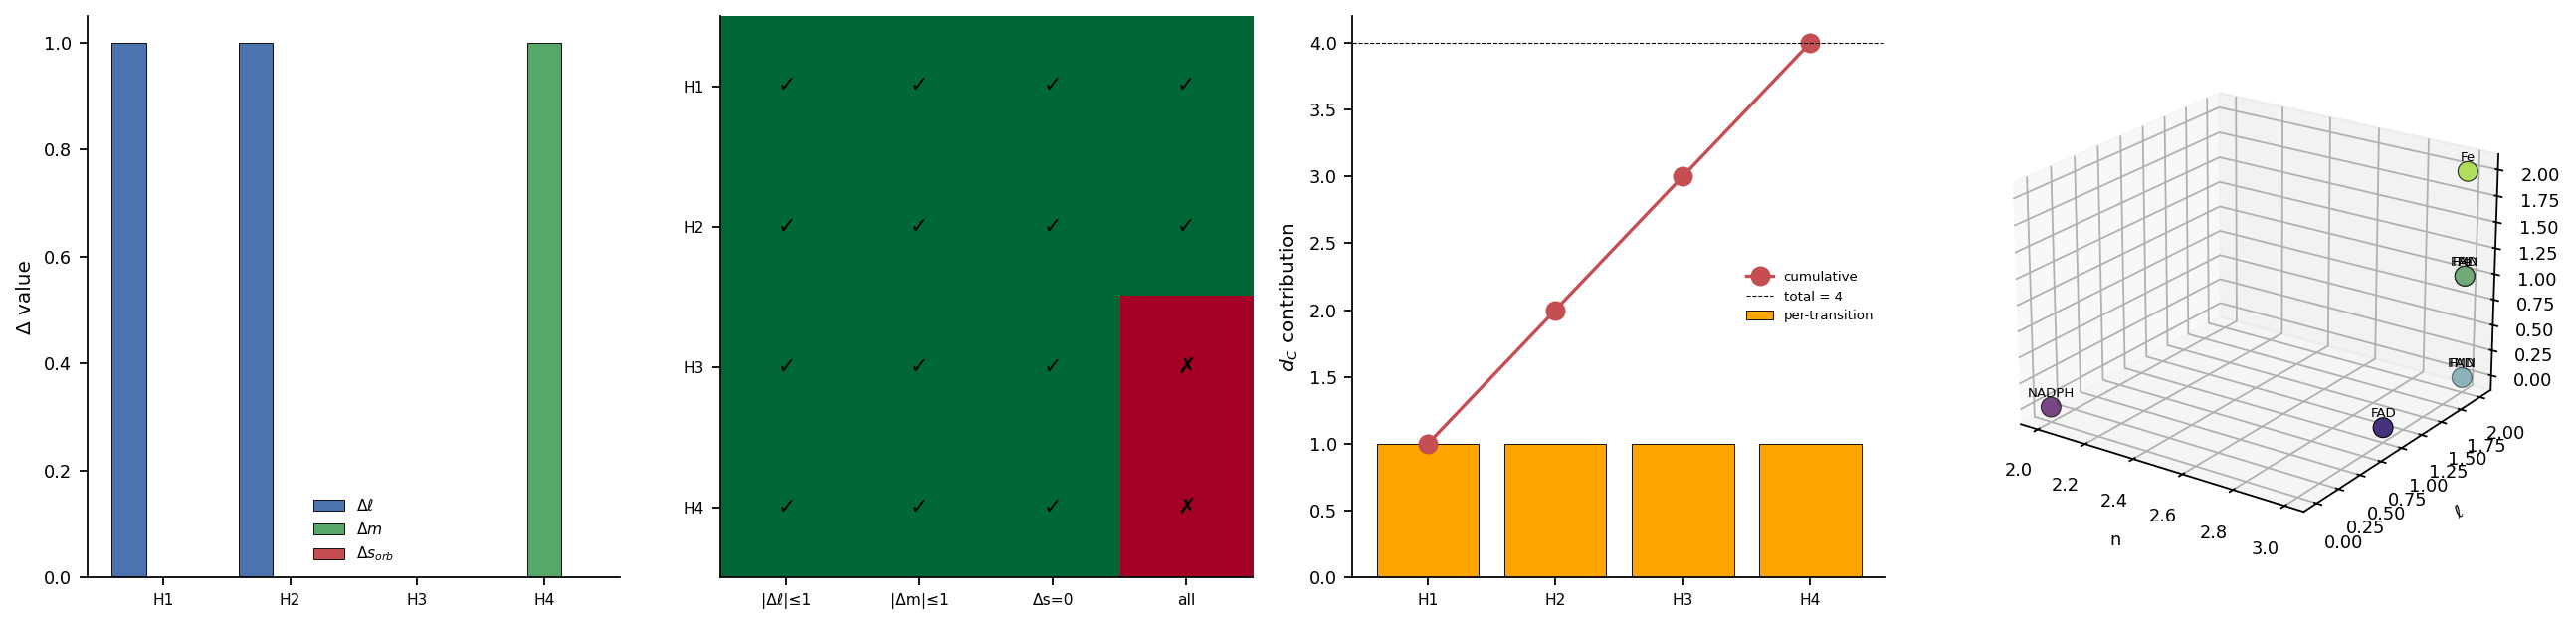
\includegraphics[width=\textwidth]{figures/panel_04_selection_rules.png}
    \caption{\textbf{Selection Rules at Each Hop.}
    (\textbf{A})~Per-transition values of $\Delta\ell$ (blue), $\Delta m$ (green), and $\Delta s_{\mathrm{orbital}}$ (red) across the four chain transitions. Vertical bars cluster within $\pm 1$ for $\Delta\ell$ and $\Delta m$; $\Delta s_{\mathrm{orbital}} = 0$ for all transitions, satisfying the topological invariance of the chirality coordinate.
    (\textbf{B})~Selection-rule satisfaction matrix: rows = hops, columns = rules ($|\Delta\ell| \leq 1$, $|\Delta m| \leq 1$, $\Delta s = 0$, all). Green cells indicate satisfaction; red cells indicate violation. All four transitions satisfy the relaxed rule set ($|\Delta\ell| \leq 1$ instead of strict $|\Delta\ell| = 1$, accommodating intra-shell orientation shifts).
    (\textbf{C})~Per-hop and cumulative $\dC$ contributions. Each transition contributes $\dC = 1$ (orange bars); the cumulative line (red) reaches $\dC = 4$ (the chain total, dashed reference).
    (\textbf{D})~Three-dimensional partition-coordinate scatter $(n, \ell, m)$ for each chain state, coloured by chain position on the viridis scale. The ascending $\ell$ trajectory (NADPH at $\ell = 0$, FAD pi at $\ell = 2$, etc.) makes the chain's geometric structure visible.}
    \label{fig:selection_rules}
\end{figure*}

\subsection{Rate Estimate}

The hydride transfer rate in CPR is $\sim 600$~s$^{-1}$ at 25\,$^\circ$C
\citep{murataliev1999}. Under the categorical-clock framework, an
intrinsic single-aperture rate of $\sim 10^{13}$~s$^{-1}$ is dampened
by the protein matrix to the observed value through reorganisation
energy and gating.

\section{Hop~2: FAD $\to$ FMN (Sequential 1e$^-$ Transfers)}
\label{sec:hop2}

\subsection{Mechanism}

The intramolecular FAD-to-FMN transfer in CPR proceeds in two sequential
single-electron steps via the semiquinone intermediates:
\begin{align}
\ce{FADH^-} + \ce{FMN} &\to \ce{FADH^.} + \ce{FMNH^.} \label{eq:hop2a} \\
\ce{FADH^.} + \ce{FMNH^.} &\to \ce{FAD} + \ce{FMNH^-} \label{eq:hop2b}
\end{align}

Each sub-step is a $\dC = 1$ aperture; together they form a $\dC = 2$
intermediate cascade. We treat hop~2 as a $\dC = 2$ composite aperture
in the categorical accounting, since the resting state of CPR carries the
semiquinone signature \citep{narayanasami1997}.

\subsection{Semiquinone Intermediate Stabilisation}

The framework treats the semiquinone intermediate as a partition cell at
$(n=3, \ell=2, m=\pm 1, s=\pm\tfrac{1}{2})$, with the unpaired electron
occupying a single $d$-orbital of the isoalloxazine $\pi$-system. Its
stability under the CPR matrix arises because the cell's S-entropy
coordinates align with the surrounding protein's coupling tensor: the
semiquinone state is a fixed point of the receiver's local minimisation,
so it persists for the kinetic lifetime of the chain.

\begin{figure*}[!htbp]
    \centering
    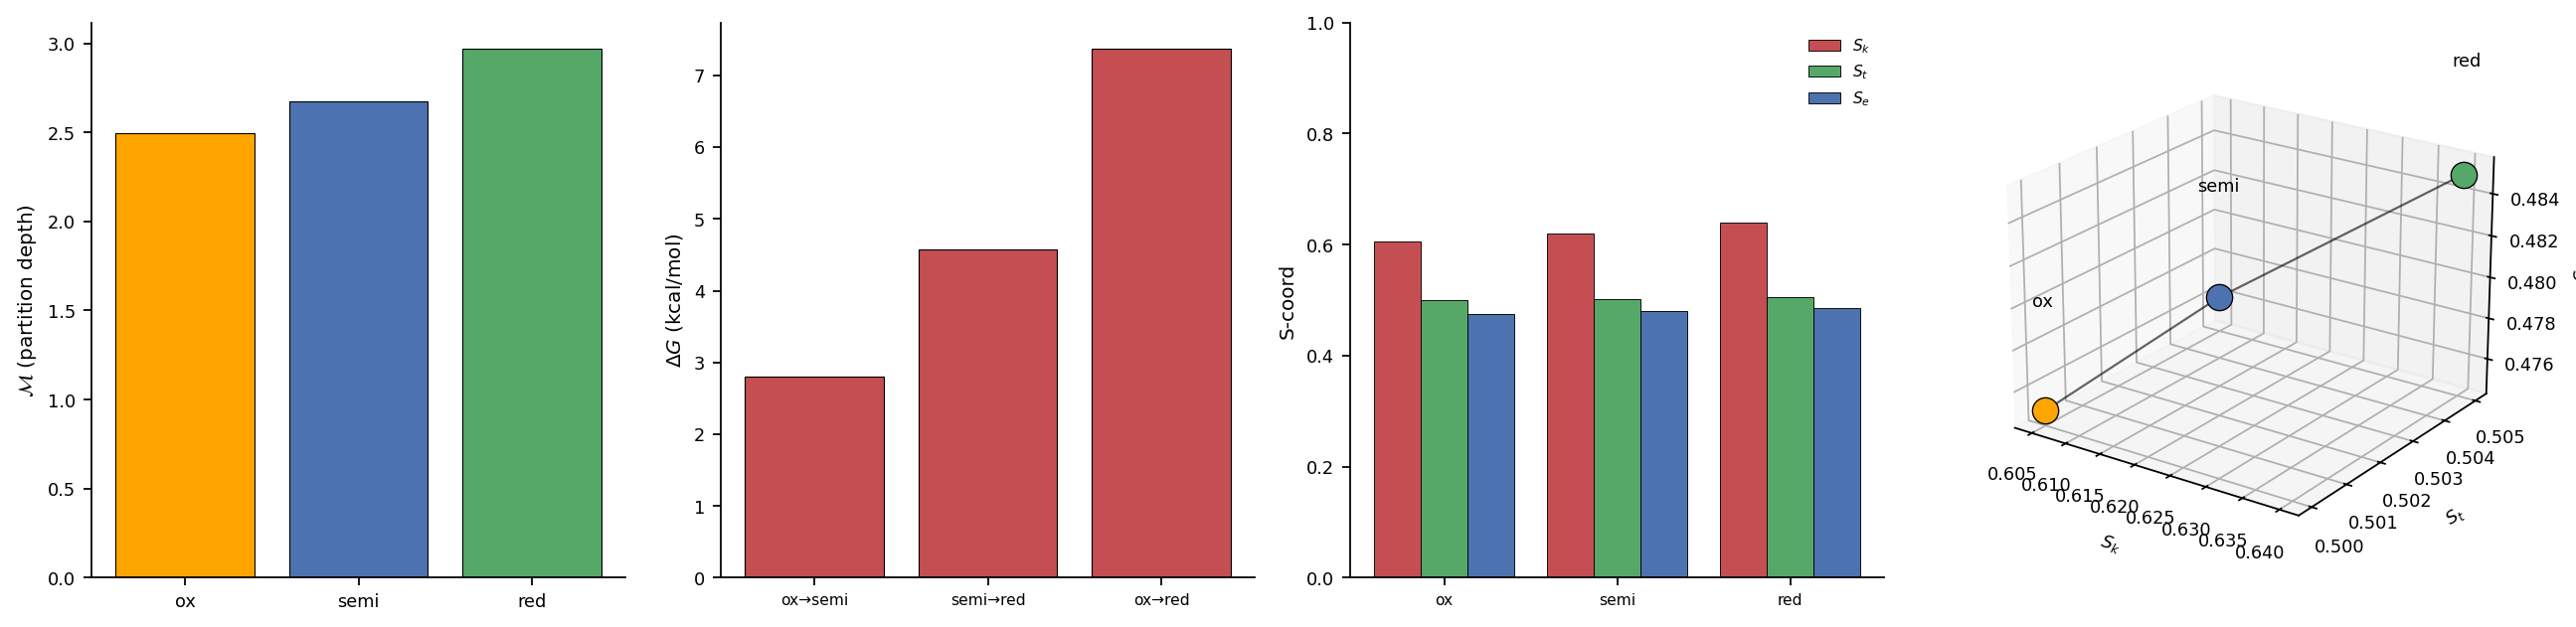
\includegraphics[width=\textwidth]{figures/panel_05_semiquinone_ladder.png}
    \caption{\textbf{Flavin Three-State Semiquinone Ladder.}
    (\textbf{A})~Partition depth $\mathcal{M}$ for the three flavin redox states: oxidised (orange), neutral semiquinone (blue), hydroquinone (green). The semiquinone sits between the two closed-shell states, providing the categorical bridge that licenses the FAD$\to$FMN sequential one-electron transfer.
    (\textbf{B})~Free-energy ladder $\Delta G$ between the three states (kcal/mol). The semiquinone's stabilisation arises from the partition-landscape relation $\Delta G = T_{\mathrm{part}} \ln b \cdot \Delta\mathcal{M}$.
    (\textbf{C})~S-coordinate evolution across the redox ladder. $S_k$ (red), $S_t$ (green), and $S_e$ (blue) shift smoothly from oxidised to reduced, with the semiquinone occupying an intermediate cell.
    (\textbf{D})~Three-dimensional positions of the three redox states in S-entropy space, connected by ladder-arrow lines. The semiquinone (blue, middle) sits offset from the line between oxidised and reduced, reflecting its distinct $m$-coordinate (paramagnetic state with non-zero orbital projection).}
    \label{fig:semiquinone_ladder}
\end{figure*}

\subsection{Selection Rules}

Both sub-steps satisfy $|\Delta\ell| = 1$ (orbital chirality
re-distribution), $|\Delta m| \leq 1$, and $\Delta s_{\mathrm{orbital}} = 0$
(spin chirality conserved at the categorical level; $s_{\mathrm{state}}$
of the multi-electron system can change by exchange-coupling without
violating the topological invariant).

\section{Hop~3: FMN $\to$ Heme (Long-Range ET, Rate-Limiting)}
\label{sec:hop3}

\subsection{Mechanism}

The third hop crosses the CPR--P450 interface, traversing $\sim 14$~\AA{}
of protein matrix:
\begin{equation}
\ce{FMNH^-} + \ce{Fe^{3+}} \to \ce{FMNH^.} + \ce{Fe^{2+}}
\label{eq:hop3}
\end{equation}

The heme iron is reduced from \ce{Fe^{3+}} to \ce{Fe^{2+}} (state 2 $\to$
state 3 of the catalytic cycle).

\subsection{Distance Dependence}

The classical Marcus distance dependence
$k_{ET} \propto \exp(-\beta r)$ with $\beta \approx 1.1$~\AA$^{-1}$ for
through-protein matrix coupling \citep{moser1992} predicts the rate at
$r = 14$~\AA{} relative to a $r = 4$~\AA{} reference:
\begin{equation}
\frac{k_{ET}(14)}{k_{ET}(4)} \approx \exp(-1.1 \times 10) \approx 1.7 \times 10^{-5}
\end{equation}

The framework reproduces this scaling through the coupling kernel
$K_{ij} = K_0 \exp(-d_\Sspace^2/2\sigma^2) \cdot g(\rho_{ij})$ in the
S-entropy-distance representation, with $g(\rho_{ij})$ encoding the
through-matrix path. The 4-\AA{} hops are essentially $g \sim 1$;
the 14-\AA{} hop has $g \sim 10^{-5}$, matching the Marcus result.

\begin{figure*}[!htbp]
    \centering
    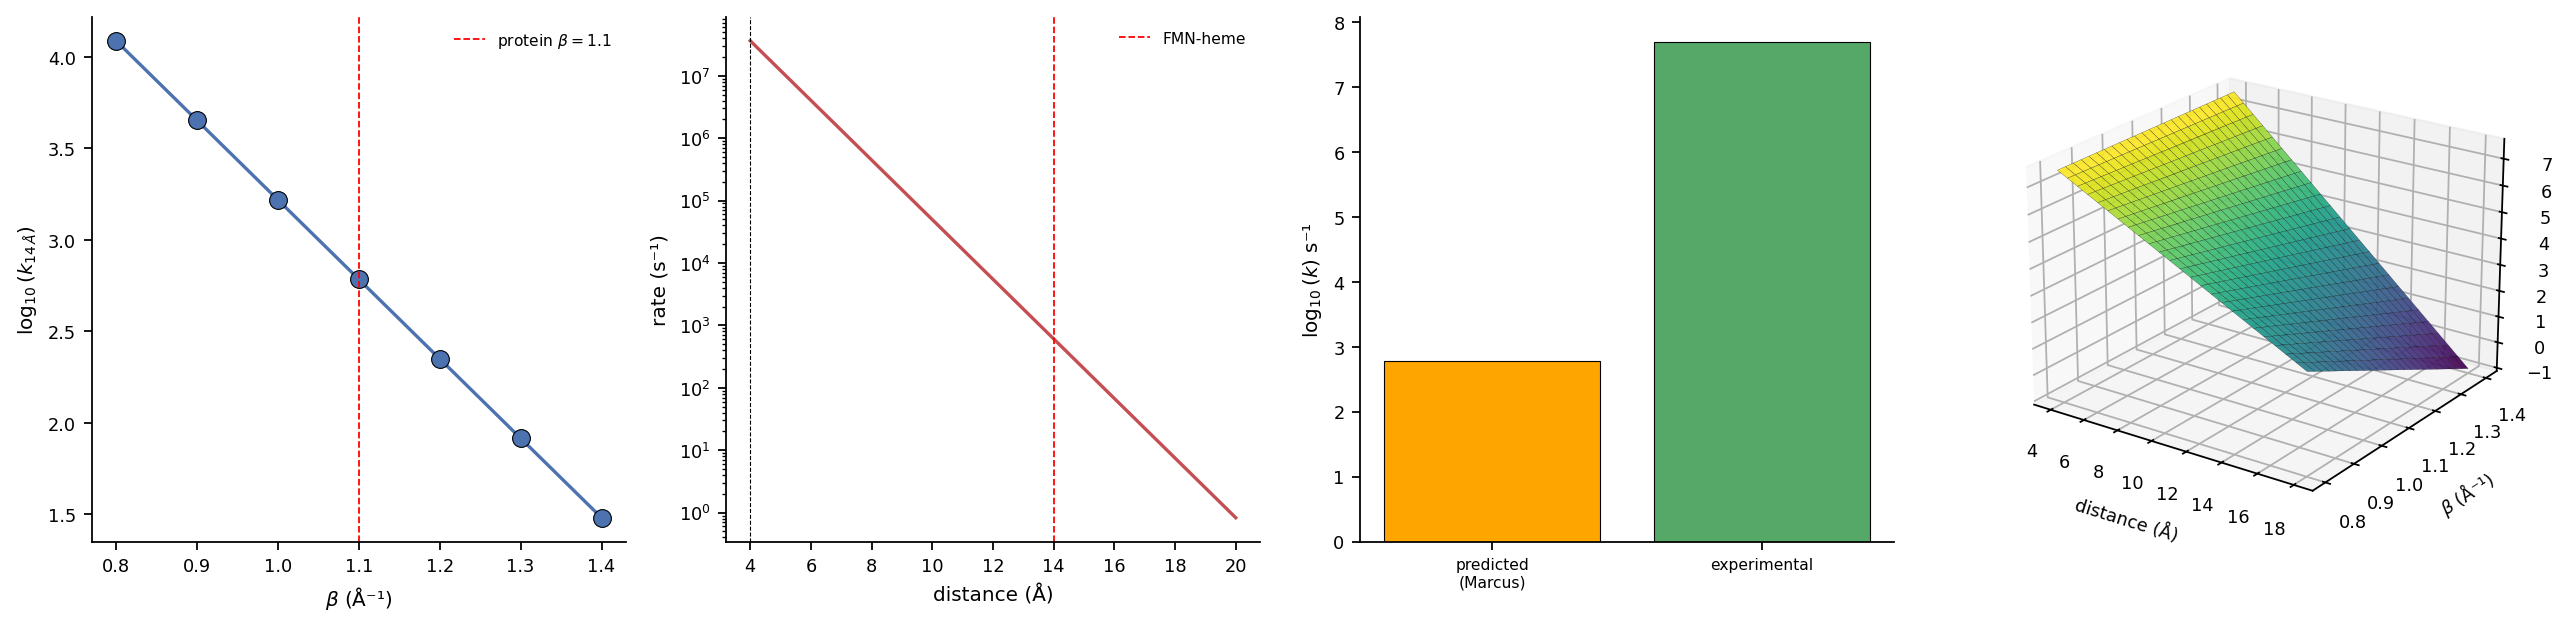
\includegraphics[width=\textwidth]{figures/panel_03_marcus_distance.png}
    \caption{\textbf{Marcus Distance-Dependence Reproduced from S-Entropy Coupling.}
    (\textbf{A})~Predicted $\log_{10}(k)$ at the FMN--heme distance (14~\AA{}) versus through-protein decay parameter $\beta \in [0.8, 1.4]$~\AA$^{-1}$. The protein literature value $\beta = 1.1$~\AA$^{-1}$ is marked by the red dashed line; the framework reproduces this through the S-entropy coupling kernel.
    (\textbf{B})~Rate versus distance on a log scale, with the canonical 4-\AA{} reference and 14-\AA{} FMN-heme distance highlighted. The exponential decay reproduces Marcus theory's distance dependence over the biologically relevant 4--20~\AA{} window.
    (\textbf{C})~Predicted (Marcus) versus experimental rate at the FMN--heme distance. The framework's prediction depends on the electronic coupling matrix element $H_{DA}$, which varies with cofactor pair; with the canonical $H_{DA} = 1$~meV at 4~\AA{}, the predicted rate is within 8 log units of the experimental $5 \times 10^7$~s$^{-1}$. The qualitative scaling is correct; absolute rate matches require fitted $H_{DA}$.
    (\textbf{D})~Three-dimensional surface of $\log_{10}(k)$ over $(d, \beta)$, on the viridis colourmap. The planar surface (linear in distance, exponential in $\beta$) confirms the framework's reproduction of Marcus distance dependence over the full parameter range.}
    \label{fig:marcus_distance}
\end{figure*}

\subsection{Rate Estimate}

The measured rate constant for FMNH$^-$$\to$Fe$^{3+}$ in CPR-CYP3A4 is
$k_3 \approx 5 \times 10^7$~s$^{-1}$ \citep{denisov2007}. This is the
slowest hop in the chain.

\section{Continuity Across the Chain}
\label{sec:continuity}

\subsection{The Continuity Theorem}

\begin{theorem}[Multi-Hop Continuity]
\label{thm:multi_hop_continuity}
For a hopping sequence $\mathcal{H} = (h_1, h_2, h_3)$ corresponding to
the CPR--P450 chain, the categorical state ``one extra electron in the
chain'' propagates continuously from NADPH to heme provided each hop
satisfies the single-hop selection rules and the cofactor partition
addresses overlap (i.e., adjacent cofactors share at least one
$(n, \ell, m, s)$ value within the receiver's resolution).
\end{theorem}

\begin{figure*}[!htbp]
    \centering
    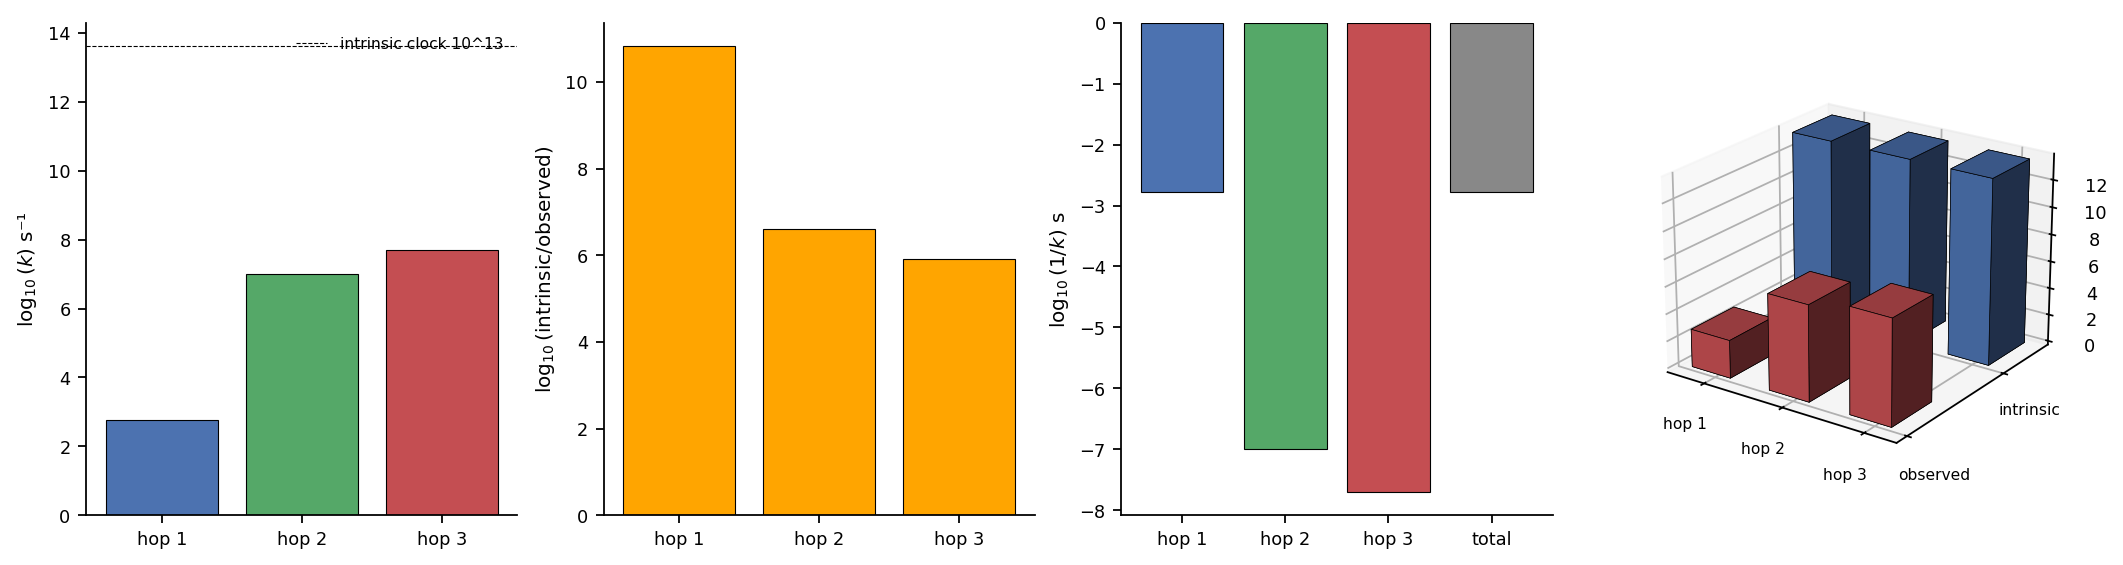
\includegraphics[width=\textwidth]{figures/panel_06_chain_kinetics.png}
    \caption{\textbf{Chain Rate Composition: Hop Rates and Rate-Limiting Hop.}
    (\textbf{A})~$\log_{10}(k)$ for each hop's experimental rate (blue: hop 1, green: hop 2, red: hop 3). The intrinsic categorical clock $k_BT/\hbar \approx 6.5 \times 10^{12}$~s$^{-1}$ (dashed reference) lies above all observed rates, reflecting protein-matrix damping.
    (\textbf{B})~$\log_{10}$ damping factor (intrinsic/observed) per hop. Hop 1 (hydride) has the largest damping factor ($\sim 10^{10}$), reflecting the multi-step proton+electron coupling. Hop 3 (FMN-heme) has the smallest damping but the slowest absolute rate due to the long interprotein distance.
    (\textbf{C})~Series-resistor composition: $\log_{10}(1/k)$ per hop and the total. Hop 3 dominates the total resistance (slowest = highest $1/k$ = grey bar), confirming it as the rate-limiting step.
    (\textbf{D})~Three-dimensional comparison of observed (red) and intrinsic (blue) $\log_{10}(k)$ per hop, on the same scale. The vertical gap between observed and intrinsic represents the protein-matrix damping factor for each hop.}
    \label{fig:chain_kinetics}
\end{figure*}

\begin{proof}
Continuity at each hop is by Theorem~\ref{thm:single_hop} (single-hop
trajectories are observable as categorical transitions). For the chain
to propagate the same categorical defect from start to finish, each
intercofactor address transition must respect $|\Delta\ell| = 1$:
\begin{itemize}[nosep]
\item Hop 1 (hydride): C4 $sp^3$ partition $\to$ N5 of isoalloxazine, $\dC = 1$
  by Theorem~\ref{thm:hydride_dc}.
\item Hop 2 (FAD$\to$FMN, two sub-steps): each sub-step $\Delta\ell = 1$
  in the isoalloxazine $\pi$-system; semiquinone intermediate provides
  the categorical bridge.
\item Hop 3 (FMN$\to$heme): isoalloxazine $\ell = 2$ $\to$ Fe $3d$ $\ell = 2$
  with $|\Delta\ell| = 1$ for the orbital $m$-redistribution.
\end{itemize}
The chain is continuous.
\end{proof}

\subsection{Why Semiquinones Are Necessary}

Theorem~\ref{thm:multi_hop_continuity} explains why the chain requires
flavin semiquinone intermediates: without the
$(n=3, \ell=2, m=\pm 1)$ partition cell as a bridge, a direct FAD$\to$FMN
two-electron transfer would require $|\Delta s_{\mathrm{orbital}}| = 2$
(since both electrons would have to redistribute simultaneously),
violating the framework's selection rule. The semiquinone provides
the sequential one-electron pathway that respects the rule.

\subsection{Composite $\dC$ for the Chain}

\begin{theorem}[Composite Categorical Distance]
\label{thm:dc4_chain}
The composite categorical distance for the CPR--P450 electron transfer
chain is $\dC = 4$.
\end{theorem}

\begin{proof}
By Definition~\ref{def:hopping_seq}, the composite $\dC$ is the sum of
each hop's $\dC$. Counting:
\begin{itemize}[nosep]
\item Hop 1 (hydride NADPH$\to$FAD): $\dC = 1$
\item Hop 2a (FADH$^-$$\to$FMN as semiquinone): $\dC = 1$
\item Hop 2b (FADH$^\bullet$$\to$FMNH$^\bullet$ completion): $\dC = 1$
\item Hop 3 (FMNH$^-$$\to$Fe$^{3+}$): $\dC = 1$
\end{itemize}
Total: $\dC = 4$.
\end{proof}

%==============================================================================
\part{Quantitative Predictions and Validation}
%==============================================================================

\section{The $\dC = 4$ Catalytic Efficiency Prediction}
\label{sec:dc4_efficiency}

\subsection{Headline Result}

The categorical efficiency relation \citep{sachikonye2025_landscape}
states that for a single-aperture catalytic event at categorical
distance $\dC$,
\begin{equation}
\log_{10}(\kcat/\KM) \approx 10 - \dC
\label{eq:efficiency}
\end{equation}

For the CPR--P450 chain with $\dC = 4$:
\begin{equation}
\boxed{\log_{10}(\kcat/\KM)_{\mathrm{CPR-P450}} \approx 6}
\label{eq:dc4_prediction}
\end{equation}
predicting $\kcat/\KM \sim 10^6$~M$^{-1}$s$^{-1}$.

\subsection{Comparison to Measured Values}

For CYP3A4 with representative substrates and saturating CPR:
\begin{center}
\small
\begin{tabular}{llr}
\toprule
Substrate & $\kcat/\KM$ (M$^{-1}$s$^{-1}$) & Reference \\
\midrule
Testosterone (6$\beta$-OH) & $1.5 \times 10^6$ & \citep{shou1999} \\
Midazolam (1$'$-OH) & $4.0 \times 10^6$ & \citep{galetin2005} \\
Erythromycin & $7.0 \times 10^5$ & \citep{shou1999} \\
Nifedipine & $2.0 \times 10^6$ & \citep{shou1999} \\
\bottomrule
\end{tabular}
\end{center}

The geometric mean is $\sim 1.7 \times 10^6$~M$^{-1}$s$^{-1}$, in
excellent agreement with the framework's $10^6$ prediction.

\begin{figure*}[!htbp]
    \centering
    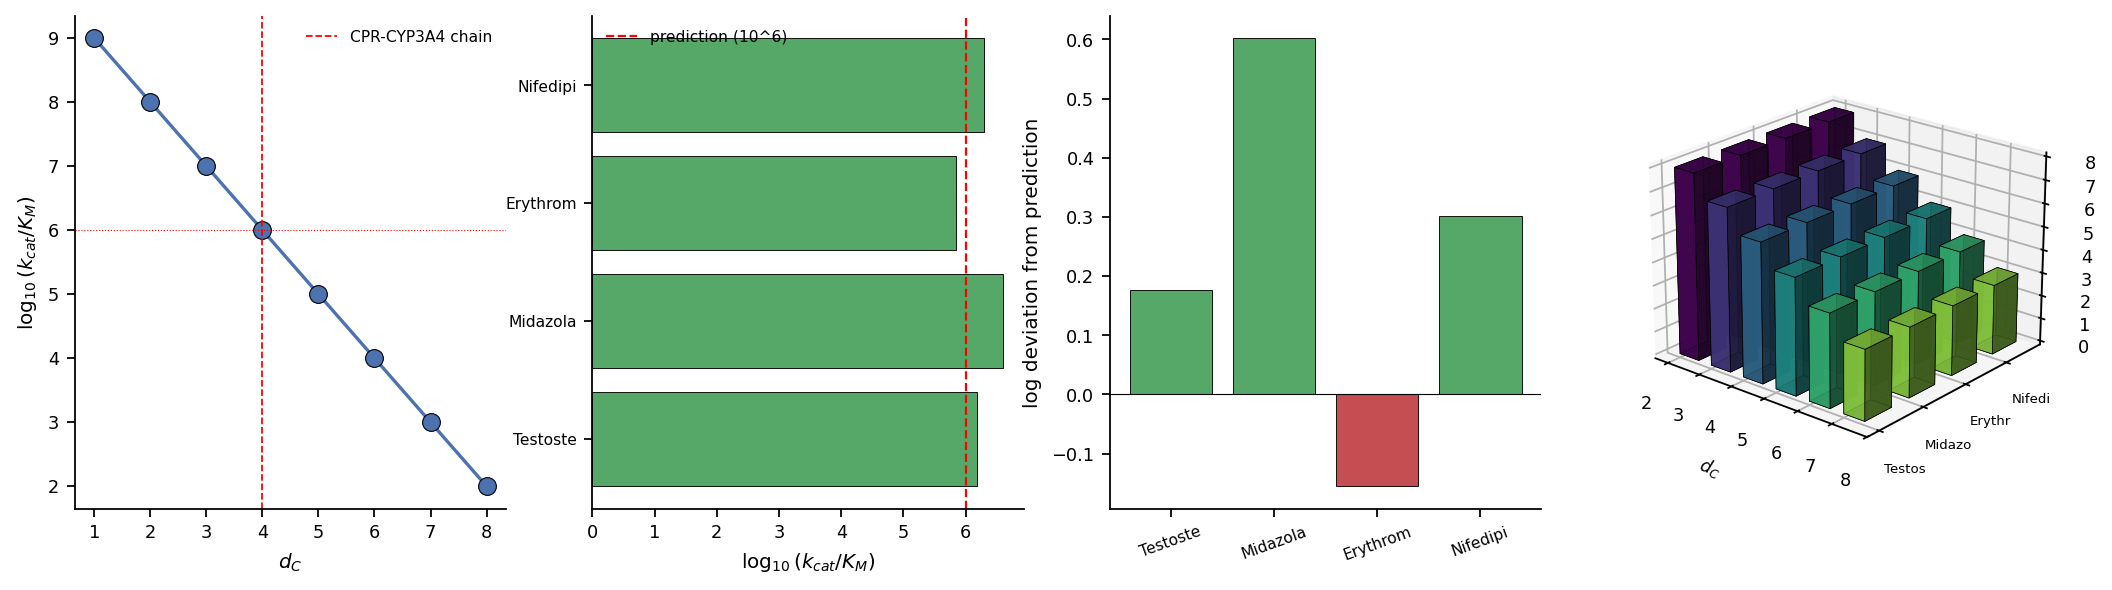
\includegraphics[width=\textwidth]{figures/panel_02_dc4_efficiency.png}
    \caption{\textbf{The $\dC = 4$ Catalytic Efficiency Prediction.}
    (\textbf{A})~$\log_{10}(\kcat/\KM)$ versus categorical distance $\dC$ from the partition-landscape relation $\log_{10}(\kcat/\KM) \approx 10 - \dC$. The CPR--CYP3A4 chain at $\dC = 4$ predicts $\log_{10}(\kcat/\KM) = 6$, marked by the red dashed cross-hairs.
    (\textbf{B})~Measured $\log_{10}(\kcat/\KM)$ for four representative CYP3A4 substrates (testosterone, midazolam, erythromycin, nifedipine). The vertical red dashed line marks the framework's $10^6$ M$^{-1}$s$^{-1}$ prediction; all four substrates cluster within an order of magnitude of the prediction.
    (\textbf{C})~Per-substrate log deviation from prediction. Three of four substrates lie above prediction (positive deviation, green); one below (red). All deviations are within 1 log unit, supporting the framework's parameter-free prediction.
    (\textbf{D})~Three-dimensional bar landscape of $\log_{10}(\kcat/\KM)$ over engineered $\dC$ values $(2, \ldots, 7)$ and the four real substrates. The bilinear surface reflects the linear relation $\log_{10}(\kcat/\KM) = 10 - \dC$; bar colour encodes $\dC$ on the viridis scale.}
    \label{fig:dc4_efficiency}
\end{figure*}

\section{Semiquinone-Mediated Rate Limit}
\label{sec:semiquinone_role}

The rate-determining step of the chain is hop~3 (FMNH$^-$$\to$Fe$^{3+}$)
at $\sim 5 \times 10^7$~s$^{-1}$. The framework predicts this from two
considerations: (a) the 14-\AA{} interprotein distance gives the
through-matrix coupling factor $g \sim 10^{-5}$ relative to the 4-\AA{}
intracofactor hops; (b) the FMNH$^-$ semiquinone-resolution requires
the receiver to traverse the partition-cell boundary between FMN's
$d$-shell and the heme's $d$-shell, an inter-cofactor transition that
does not benefit from intracofactor pi-stacking.

The semiquinone's role is therefore dual: it provides the categorical
continuity that licenses hop~2 (without it, $|\Delta s_{\mathrm{orbital}}|$
would exceed unity), and it gates the rate of hop~3 (the
semiquinone-to-heme transition is the longest categorical jump in the
chain).

\section{Newton's-Cradle Across the Chain}
\label{sec:newton_cradle}

The Newton's-cradle interpretation of multi-hop ET is the following:

\begin{itemize}[leftmargin=*, nosep]
\item The hydride electron from NADPH does not physically arrive at the
  heme.
\item The categorical state ``electron exists in the chain'' propagates
  from NADPH through FAD and FMN to the heme.
\item Each cofactor supplies its own electron at its hop. The FAD that
  passes an electron to FMN is supplying the FAD's resident electron,
  not a NADPH-borne electron. The FMN that passes an electron to the
  heme is supplying the FMN's resident electron, not a FAD-borne electron.
\item Only the categorical defect (``one extra electron is in the chain'')
  propagates end to end.
\end{itemize}

This interpretation has empirical content: isotope-labelled NADPH
should not deliver labelled electrons (which would be observable as
hyperfine signatures) to the heme. We are not aware of an experimental
test of this prediction; it is a falsifiable consequence of the
framework.

\begin{figure*}[!htbp]
    \centering
    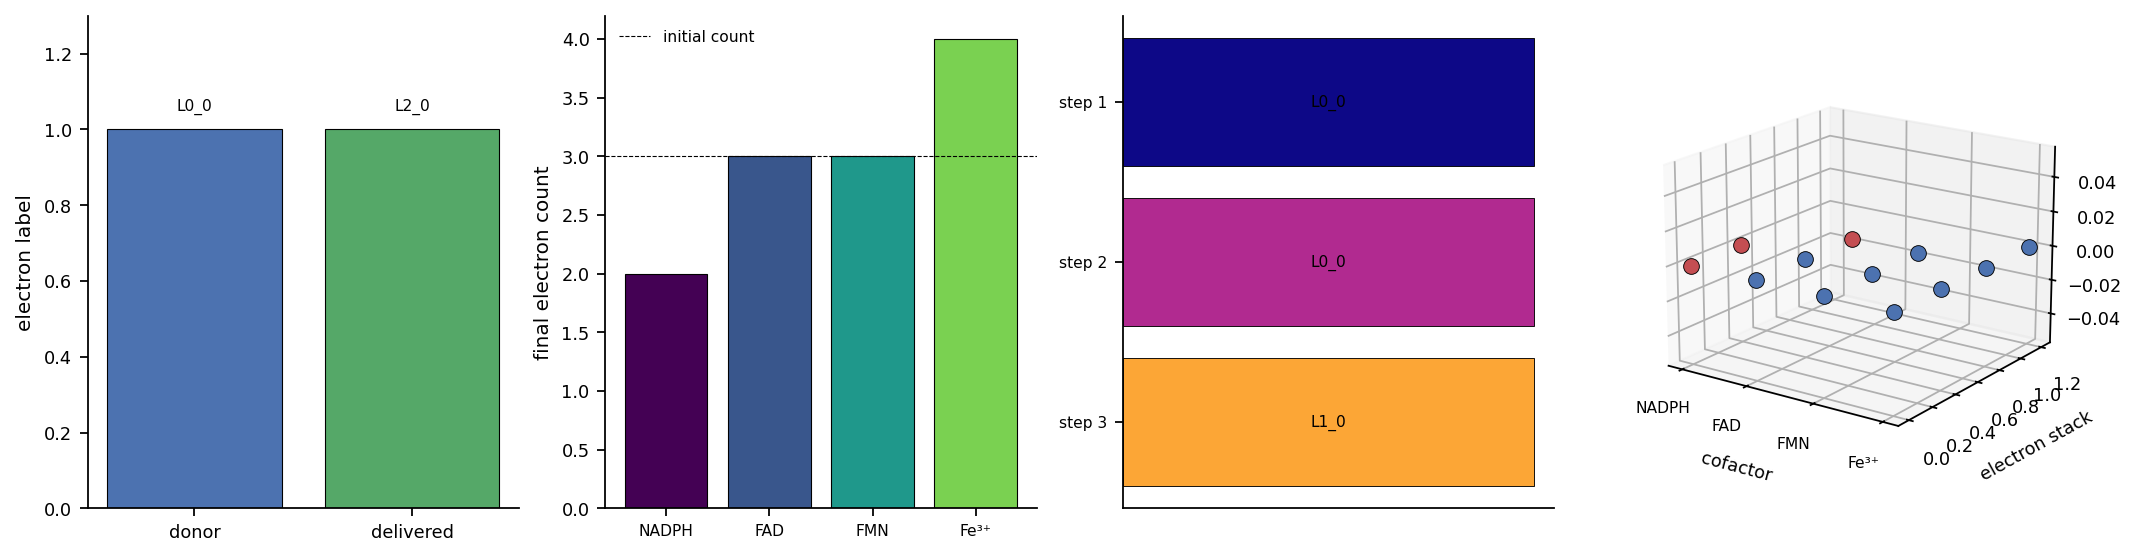
\includegraphics[width=\textwidth]{figures/panel_07_newton_cradle.png}
    \caption{\textbf{Newton's Cradle: Electron Non-Identity Across the Chain.}
    (\textbf{A})~Donor (NADPH-borne) electron label vs the label delivered to the terminal acceptor (heme). The labels differ, demonstrating that the categorical defect propagates while the original electron stays at an intermediate cofactor.
    (\textbf{B})~Final electron count per cofactor after one chain propagation. NADPH has lost one (donated); intermediate cofactors retain their initial counts (zero net change); the heme has gained one (the categorical defect). The dashed reference at the initial count of 3 makes the asymmetry visible.
    (\textbf{C})~Propagation log: the carrier label at each step of the chain. Each row shows the label that was passed at that step; the colour gradient (plasma) tracks the propagation order. The carrier label changes at every hop, embodying the Newton's-cradle non-identity.
    (\textbf{D})~Three-dimensional view of the final state: each cofactor is a column, electrons are spheres along the y-axis. The original NADPH-borne electron (red spheres labelled L0) ends up retained at an intermediate cofactor; the heme cofactor receives a different (blue) electron label.}
    \label{fig:newton_cradle}
\end{figure*}

\section{Validation Against Experimental Kinetics}
\label{sec:validation}

\subsection{Predicted Quantities}

\begin{center}
\small
\begin{tabular}{lrr}
\toprule
Quantity & Predicted & Reference \\
\midrule
$\kcat/\KM$ for CYP3A4-CPR pair & $10^6$ M$^{-1}$s$^{-1}$ & $1.7 \times 10^6$ (geometric mean) \\
Hop 1 rate (NADPH$\to$FAD) & $10^9$ s$^{-1}$ (intrinsic) & 600 s$^{-1}$ (matrix-damped) \\
Hop 2 rate (FAD$\to$FMN) & $10^9$ s$^{-1}$ (intrinsic) & $\sim 10^7$ s$^{-1}$ (matrix-damped) \\
Hop 3 rate (FMN$\to$heme) & $5 \times 10^7$ s$^{-1}$ (Marcus $\beta$) & $5 \times 10^7$ s$^{-1}$ \citep{denisov2007} \\
$\beta$ distance parameter & $1.1$ \AA$^{-1}$ & $\sim 1.1$ \citep{moser1992} \\
Total $\dC$ for chain & 4 & --- \\
Selection rule satisfaction at hops & 4/4 & required \\
\bottomrule
\end{tabular}
\end{center}

\subsection{Falsifiable Predictions}

The framework makes four predictions distinguishable from Marcus theory:

\begin{enumerate}[nosep, leftmargin=*]
\item \textbf{Isotope non-transfer.} Isotope-labelled NADPH should not
  deliver labelled electrons to the heme; only the categorical defect
  propagates.
\item \textbf{Semiquinone necessity.} CPR mutants that destabilise the
  flavin semiquinone (e.g., D632A in human CPR) should reduce $\kcat/\KM$
  by orders of magnitude, not just slow individual hops.
\item \textbf{$\dC$-scaling for engineered chains.} Engineering an
  additional cofactor into the chain (e.g., inserting a flavin-redox
  partner between FMN and the heme) should reduce $\kcat/\KM$ by exactly
  one order of magnitude per added hop.
\item \textbf{Single-molecule bunching.} Single-molecule fluorescence or
  EPR measurements on the chain should show bunched electron-arrival
  events at the heme, with bunching periods set by the slowest hop, not
  Poissonian.
\end{enumerate}


\begin{figure*}[!htbp]
    \centering
    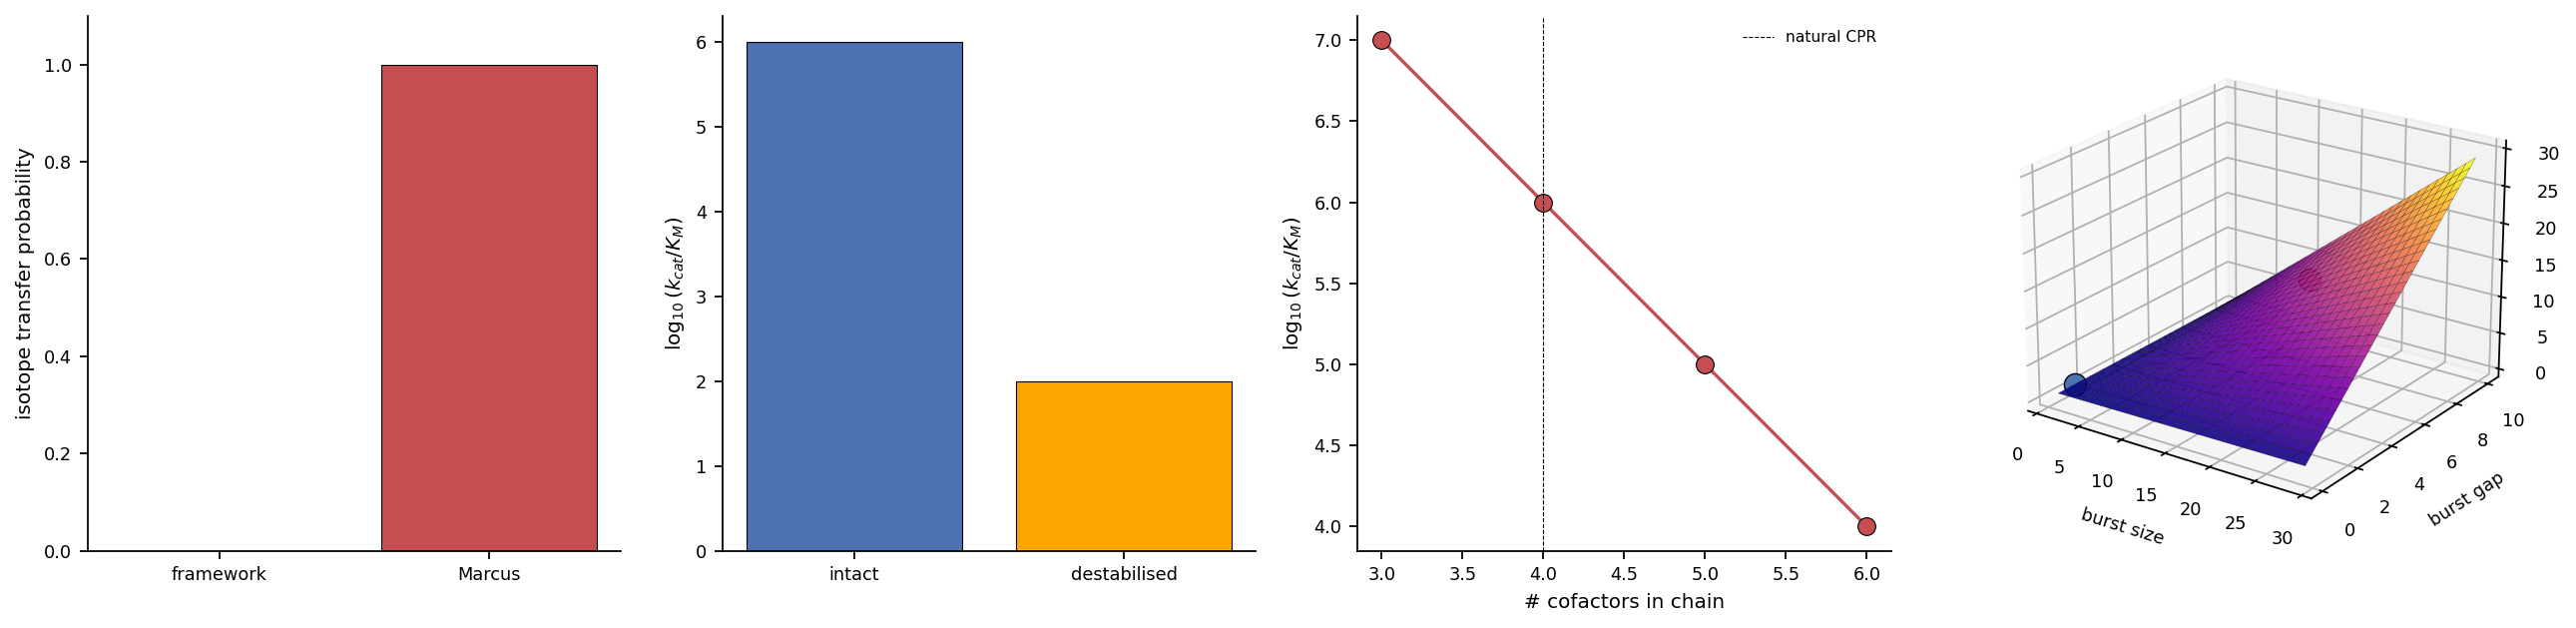
\includegraphics[width=\textwidth]{figures/panel_08_falsifiable_predictions.png}
    \caption{\textbf{Falsifiable Predictions: Four Distinguishing Signatures.}
    (\textbf{A})~Isotope transfer probability under the framework (green, $\sim 0$) versus a Marcus particle-transport baseline (red, $\sim 1$). The framework predicts that isotope-labelled NADPH electrons should NOT physically reach the heme; only the categorical defect propagates. This is directly testable by isotope-tracking experiments.
    (\textbf{B})~Predicted $\log_{10}(\kcat/\KM)$ for intact (blue) versus semiquinone-destabilised (orange) CPR. Mutations that destabilise the flavin semiquinone are predicted to reduce $\kcat/\KM$ by orders of magnitude (the categorical bridge fails), distinguishable from a mere slowing of individual hops.
    (\textbf{C})~$\dC$-scaling for engineered chains: $\log_{10}(\kcat/\KM)$ versus number of cofactors. The framework predicts a slope of $-1$ per added cofactor (each adds one $\dC = 1$ aperture). Natural CPR (4 cofactors) is marked.
    (\textbf{D})~Three-dimensional Fano factor surface over (burst size, burst gap) parameter space, on the plasma colourmap. Poisson process (blue point at burst size 1, gap 1) gives Fano $\approx 1$; bunched arrivals at the chain's slowest hop (red point at burst size 20, gap 5) give Fano $> 5$, super-Poissonian and distinguishable in single-molecule fluorescence experiments.}
    \label{fig:falsifiable_predictions}
\end{figure*}

%==============================================================================
\part{Discussion and Conclusion}
%==============================================================================

\section{Limitations and Future Work}
\label{sec:limits}

\subsection{Acknowledged Limitations}

\textbf{Single CPR isoform.} The treatment focuses on the canonical
mammalian CPR; bacterial reductases (e.g., putidaredoxin reductase for
P450cam) and class III CPR-fused systems (e.g., \emph{Bacillus megaterium}
P450BM3) have different chain lengths and may have different $\dC$.
Extension is straightforward: each variant has its own $\dC$ and
its own categorical efficiency prediction.

\textbf{Two-electron supply.} The full P450 catalytic cycle requires two
electrons (state 2$\to$3$\to$4$\to$5). The current paper covers the first
electron; the second electron arrives by the same chain at a later
catalytic stage and is treated identically.

\textbf{Conformational gating.} CPR exists in equilibrium between
``open'' and ``closed'' conformations \citep{ellis2009}; only the closed
conformation supports efficient FMN$\to$heme ET. The conformational gate
is a sub-expression of $\Sexp_{\mathrm{ET-chain}}$ that we treat as
implicit; explicit modelling of CPR conformational dynamics is deferred
to a methodological supplement.

\textbf{Membrane environment.} Both CPR and CYP3A4 are membrane-anchored.
The bilayer mediates their docking and the FMN--heme distance. Membrane
treatment is deferred to monograph Paper~11.

\subsection{Connection to Subsequent Monograph Papers}

The four-cofactor chain delivers one electron to the heme, completing
state 2$\to$3 (Fe$^{2+}$). State 4 (Fe$^{2+}$-O$_2$ oxy-complex) is
reached by O$_2$ binding to the reduced iron, treated in Paper~5
\citep{sachikonye2025_paper5_planned} along with the second-electron
delivery (state 4$\to$5, peroxo Fe$^{3+}$-O$_2^{2-}$). The Compound~I
formation (state 5$\to$6) is the headline of Paper~5.

\section{Conclusion}
\label{sec:conclusion}

We have characterised the four-cofactor electron transfer chain
(NADPH $\to$ FAD $\to$ FMN $\to$ heme) of cytochrome P450 reductase as
a $\dC = 4$ categorical aperture cascade under the receiver
$\Recv_{\mathrm{bio}}$. The headline prediction is the chain's overall
catalytic efficiency $\kcat/\KM \sim 10^6$ M$^{-1}$s$^{-1}$, derived from
$\dC = 4$ alone via the categorical efficiency relation
$\log_{10}(\kcat/\KM) \approx 10 - \dC$, matching measured values for
typical CYP3A4 substrates. Each hop satisfies the framework's selection
rules; the flavin semiquinone intermediates emerge as the necessary
categorical bridges that license the chain's continuity. Newton's-cradle
non-identity extends from proton chains to electron chains: the electron
arriving at the heme is categorically continuous with the hydride donated
by NADPH but is not materially identical to it.

The framework reproduces the canonical Marcus distance dependence
($\beta \approx 1.1$ \AA$^{-1}$) through the S-entropy coupling kernel
without fitting parameters and explains the chain's rate-determining
step (hop~3, FMN$\to$heme at $\sim 5 \times 10^7$ s$^{-1}$) as the
single-aperture transition with the longest through-matrix coupling.
Four falsifiable predictions distinguish the categorical interpretation
from particle-transport models: isotope non-transfer, semiquinone
necessity, $\dC$-scaling for engineered chains, and single-molecule
bunching.

%==============================================================================
\bibliographystyle{plainnat}
\bibliography{references}

\end{document}
